\begin{frame}
\frametitle{Memory Controller (Old, 200x)}
\begin{center}
  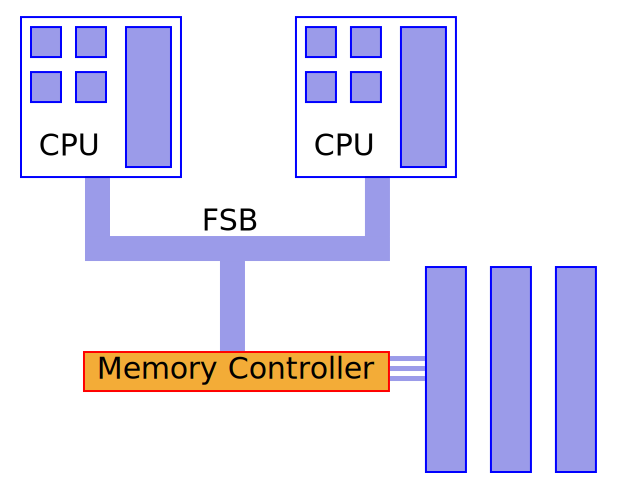
\includegraphics[width=0.8\linewidth]{fsb.png}
\end{center}
\end{frame}

\begin{frame}
\frametitle{Memory Controller (New, 201x)}
\begin{center}
  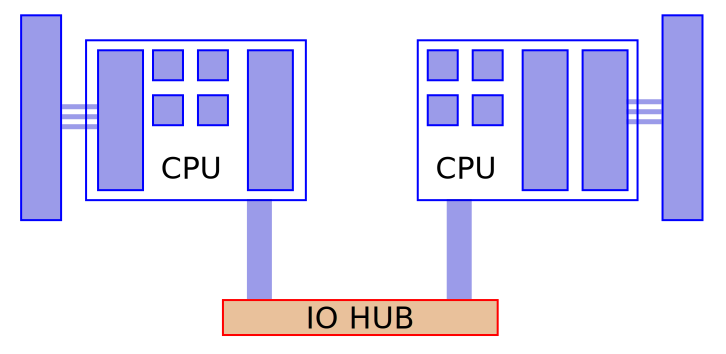
\includegraphics[width=0.8\linewidth]{qpi.png}
\end{center}
\begin{itemize}
  \item CPU видит память через Memory Controller
  \begin{itemize}
    \item подключите к Memory Controller хоть чайник, CPU будет считать его
    памятью.
  \end{itemize}
\end{itemize}
\end{frame}

\begin{frame}
\frametitle{Неоднородность памяти}
\begin{itemize}
  \item Запросы в "память" могут переадресовываться устройствам и иметь побочные
  эффекты:
  \begin{itemize}
    \item например, запись по адресу 0xb8000 приводит к выводу на экран;
    \item обращение по адресу 0xfee00000 переадресуется Local APIC-у;
    \item обращение по адресу 0xfec00000 переадресуется IO APIC-у.
  \end{itemize}
  \item Память по каким-то адресам может отсутсвовать впринципе:
  \begin{itemize}
    \item регионы зарезервированные для устройств отображенных в память и
    неиспользованные;
    \item ISA Hole, участки зарезервированные для PCI и прочих устройств.
  \end{itemize}
\end{itemize}
\end{frame}

\begin{frame}
\frametitle{Карта памяти}
\begin{itemize}
  \item ОС управляет памятью и должна иметь информацию о доступной памяти:
  \begin{itemize}
    \item чтобы настроить алокаторы памяти;
  \end{itemize}
  \item разные системы используют разные интерфейсы для получения карты памяти:
  \begin{itemize}
    \item BIOS, INT 0x15 функция 0xe820;
    \item UEFI, GetMemoryMap();
    \item multiboot (другой загрузчик) может предоставлять карту памяти;
    \item карта памяти может передаваться ОС как аргумент при старте;
    \item \href{https://firmware.intel.com/sites/default/files/resources/A_Tour_Beyond_BIOS_Memory_Map_in\%20UEFI_BIOS.pdf}{A tour beyond BIOS memory map in UEFI BIOS}.
  \end{itemize}
\end{itemize}
\end{frame}
